
%%%%%%%%%%%%%%%%%%%%%%% file typeinst.tex %%%%%%%%%%%%%%%%%%%%%%%%%
%
% This is the LaTeX source for the instructions to authors using
% the LaTeX document class 'llncs.cls' for contributions to
% the Lecture Notes in Computer Sciences series.
% http://www.springer.com/lncs       Springer Heidelberg 2006/05/04
%
% It may be used as a template for your own input - copy it
% to a new file with a new name and use it as the basis
% for your article.
%
% NB: the document class 'llncs' has its own and detailed documentation, see
% ftp://ftp.springer.de/data/pubftp/pub/tex/latex/llncs/latex2e/llncsdoc.pdf
%
%%%%%%%%%%%%%%%%%%%%%%%%%%%%%%%%%%%%%%%%%%%%%%%%%%%%%%%%%%%%%%%%%%%


\documentclass[runningheads,a4paper]{llncs}

\usepackage{amssymb}
\setcounter{tocdepth}{3}
\usepackage{graphicx}

\usepackage{url}
\urldef{\mailsa}\path|{alfred.hofmann, ursula.barth, ingrid.haas, frank.holzwarth,|
\urldef{\mailsb}\path|anna.kramer, leonie.kunz, christine.reiss, nicole.sator,|
\urldef{\mailsc}\path|erika.siebert-cole, peter.strasser, lncs}@springer.com|    
\newcommand{\keywords}[1]{\par\addvspace\baselineskip
\noindent\keywordname\enspace\ignorespaces#1}

\begin{document}

\mainmatter  % start of an individual contribution

% first the title is needed
\title{Sistema de Recuperación de Información}

% a short form should be given in case it is too long for the running head
\titlerunning{Sistema de Recuperación de Información}

% the name(s) of the author(s) follow(s) next
%
% NB: Chinese authors should write their first names(s) in front of
% their surnames. This ensures that the names appear correctly in
% the running heads and the author index.
%
\author{Carlos Rafael Ortega Lezacano \and Eric Martín García \\ Grupo C511}
%
\authorrunning{Sistema de Recuperación de Información}
% (feature abused for this document to repeat the title also on left hand pages)

% the affiliations are given next; don't give your e-mail address
% unless you accept that it will be published
\institute{Universidad de la Habana}

%
% NB: a more complex sample for affiliations and the mapping to the
% corresponding authors can be found in the file "llncs.dem"
% (search for the string "\mainmatter" where a contribution starts).
% "llncs.dem" accompanies the document class "llncs.cls".
%

\toctitle{Sistema de Recuperación de Información}
\tocauthor{Authors' Instructions}
\maketitle

\section{Introducción}

Los sistemas de recuperación de información brindan un manejo efectivo de un conjunto considerable de datos, poder realizar consultas a un conjunto de documentos por parte de los usuarios es una característica fundamental en estos, hoy en día son de vital importancia para todos, a diario realizamos búsquedas en Google, ResearchGate entre otros sitios los cuales cuentan con un volumen de información considerable. 

La primera descripción de una computadora que buscaba información fue propuesta por Holmstrom en 1948, detallando una mención temprana de la computadora Univac. Los sistemas automatizados de recuperación de información se introdujeron en la década de 1950. En la década de 1960, Gerard Salton en Cornell formó el primer gran grupo de investigación de recuperación de información. En la década de 1970, se había demostrado que diferentes técnicas de recuperación funcionaban bien en corpus de texto pequeños, como la colección Cranfield (varios miles de documentos). Los sistemas de recuperación a gran escala, como el sistema Lockheed Dialog, se empezaron a utilizar a principios de la década de 1970. 

En este escrito analizaremos la implementación realizada de un IRS, primeramente exponiendo los conceptos teóricos empleados para el diseño del sistema, las herramientas usadas para el procesamiento de los corpus y por último realizaremos una evaluación del sistema. 

\section{Diseño del Sistema}

Un sistema de recuperación de información (IRS) se compone por el cuádruplo $<D,\ Q,\ F,\ R(q_j, d_j)>$, donde $D$ es un conjunto de documentos que conforman un corpus, $Q$ es un conjunto compuesto por representaciones lógicas de los pedidos que el usuario realiza al sistema, $F$ es un framework para modelar los documentos del corpus y $R$ es una función de orden donde para cada par, consulta $q_j$ y documento $d_j$, le asigna un valor acorde a la relevancia del documento para esa consulta. El proceso de interacción de un sistema con un usuario sigue el siguiente comportamiento: Primeramente el usuario realiza una consulta (un elemento de $Q$), esta pasa al motor de búsqueda, este es un componente importante para el sistema ya que realiza las representaciones de los documentos\footnote{En nuestro sistema se usa un IRS vectorial por tanto la representación interna se realiza mediante vectores cuyas componentes son pesos asociados a la entidad resultante del preprocesamiento}, además de representar la consulta en formato interno, el sistema dará como resultado una lista ordenada por relevancia de los documentos del corpus. Analizaremos a continuación las consultas, la composición del motor de búsqueda y como clasifica los documentos para dar una salida acorde a la relevancia. En nuestro caso el sistema va enfocado en la búsqueda de documentos, un documento tiene varias características, dos de las más comunes y útiles a la hora de realizar búsquedas es el título y el cuerpo.

\subsection*{Motor de Búsqueda}

El motor de búsqueda implementa un modelo de recuperación de información, además en este se realiza el preprocesado de los documentos para su representación interna. Cada consulta realizada al sistema es almacenada para poder realizar medidas de precisión y efectividad al sistema. También es el encargado de construir el ranking de relevancia de los documentos del corpus acorde a la consulta de entrada.

\subsubsection{Preprocesamiento:} 

Para representar los documentos primeramente es necesario realizar un preprocesado, en nuestro sistema procederemos de forma simple, empleando recursos del procesamiento de lenguaje natural para modificar los documentos y luego poder vectorizar. Las siguientes transformaciones son realizadas para cada documento del corpus:

\begin{enumerate}
	\item \textbf{Tokenizar el documento:} Primeramente es necesario crear la representación básica de un documento, la división en tokens, de tal forma que podamos realizar procesamientos más avanzados sobre el texto. Desde esta etapa del preprocesamiento podemos llevar a minúscula todos los caracteres de las palabras, eliminar símbolos y signos de puntuación. \\
	
	\item \textbf{Eliminación de \textit{stopwords}:} Las \textit{stopwords} como sabemos son palabras vacias de significado, las cuales pueden servir de nexo entre entidades o funcionan como modificadores. Si incluimos estas palabras en la representación del documento se puede afectar precisión del modelo, debido a la alta frecuencia que poseen estas palabras en los textos. \\
	
	\item \textbf{Stemming:} Este método busca relacionar palabras con igual significado
	pero que difieren en cuanto a la escritura debido a  que presentan prefijos o
	sufijos. En este caso no usaremos lematización, la cual es común aplicar luego del stemming.
\end{enumerate} 

Estas técnicas son las empleadas por el sistema para obtener un conjunto de textos formados por entidades con un significado y peso correcto para empezar a construir el modelo, pero antes de definir el modelo es necesario definir como serán estas entidades y que representación interna tendrán. Se eligió emplear los tokens como entidad del sistema, de esta forma se construye una colección con el siguiente formato:  \\

\noindent
{\it Representación del titulo y el cuerpo del documento preprocesado}
\begin{verbatim}
	    corpus: {
                   [id: n,
                   'title': Tokenize(doc_title),
                   'body': Tokenize(doc_body),
                   ],
                   ...
             }
\end{verbatim}
%
\noindent

\subsubsection{Vectorización:} Una vez que tenemos los tokens es necesario realizar una vectorización, así podemos tener una entrada correcta para el modelo, emplearemos para ello TF-IDF. Para calcular los valores de frecuencia  emplearemos el título y el cuerpo del documento juntos, sin realizar distinción, o sea el título podría ser una oración más del texto.

\paragraph*{TF-IDF:} Es una técnica para cuantificar una palabra en documentos, generalmente calculamos un peso para cada palabra que significa la importancia de la palabra en el documento y corpus. Este método es una técnica ampliamente utilizada en recuperación de información y minería de textos. Esta se representa por $w(t_i, d_j)$ donde $t_i$ es un término del documento $d_j$. \\

El TF-IDF se compone de dos conceptos fundamentales que se apoyan en el procesamiento de los documentos, el TF (Frecuencia de Termino) y el IDF (Frecuencia Inversa de Documento).

\paragraph*{TF:} Mide la frecuencia de una palabra en un documento. Esto depende en gran medida de la longitud del documento y de la generalidad de la palabra, por ejemplo, una palabra muy común como "casa" puede aparecer varias veces en un documento. Como los documentos pueden tener una longitud variable entonces contar simplemente las palabras podría dar prioridad a documentos de mayor tamaño, por eso es que se divide la cantidad de ocurrencias por el número total de palabra del documento $N(d_j)$. TF es individual para cada documento y palabra, por lo tanto, podemos formular TF de la siguiente manera:

\begin{equation}
	f_s(t_i, d_j) = \frac{C(t_i, d_j)}{N(d_j)}
\end{equation}

Donde $C(t_i, d_j)$ representará la cantidad de ocurrencias del término en el documento. Recordemos que estamos vectorizando los documentos por tanto es necesario introducir el concepto de \textbf{vocabulario}, este es un conjunto formado por todas las palabras del corpus, o sea todas las palabras que hay en cada documento, de esta forma garantizamos que los vectores para cada documento tengan igual dimensión. Cada componente tendrá el valor de frecuencia asociado para esa palabra, este valor estará en el intervalo $[0,1]$. Esta ponderación de las palabras beneficia a palabras comunes que se repiten en los documentos, Por lo tanto es necesario incluir una definición de frecuencia para palabras menos comunes. Antes de definir IDF es necesario definir Frecuencia de Documento, ya que su inversa es IDF.

\paragraph*{DF:} Esta mide la importancia del documento en todo el conjunto de corpus. DF es el recuento de apariciones del término $t_i$ en el conjunto de documentos $D$. En otras palabras, DF es el número de documentos en los que está presente la palabra. Consideraremos una ocurrencia si el término consta en el documento al menos una vez, no necesitamos saber el número de veces que el término está presente. 

Como en el caso de TF también normalizamos dividiendo por el número total de documentos. Nuestro principal objetivo es conocer la informatividad de un término poco común, para eso invertimos DF.

\paragraph*{IDF:} Es la inversa de la frecuencia del documento que mide la informatividad del término $t_i$. Cuando calculemos el IDF, será muy bajo para las palabras más frecuentes y mayor para las menos comunes. Como es posible que el DF sea cero entonces es necesario realizar algunas modificaciones para no dividir entre 0, además si el corpus es grande podemos entonces obtener un valor alto, que no es de utilidad, por lo tanto emplearemos  una función de crecimiento más lento para suavizar IDF.

\begin{equation}
	\overline{d}_s(t_i) = \log{\frac{|D|}{d_s(t_i) + 1}}
\end{equation}

Ahora combinemos ambas frecuencias, de esta forma tendremos una relación entre términos de mucha ocurrencia con respecto a aquellos de baja frecuencia en los documentos.

\begin{equation}
	w(t_i, d_j) = f_s(t_i, d_j) \cdot \log{\frac{|D|}{d_s(t_i) + 1}}
\end{equation}

Hasta el momento se ha expuesto el concepto de TF-IDF para documentos pero ignorando si tienen título o no. Los textos que conforman el corpus del motor de búsqueda tienen diversas características y hemos elegido el título y el cuerpo para realizar el procesamiento y representación, por lo tanto debemos determinar cual de estos es más importante a la hora  dar un valor de relevancia a un documento, para ello definamos el parámetro $\alpha$ el cual define cuanto peso le damos al título a la hora de calcular la relevancia, de esta forma tendríamos que determinar los valores de TF-IDF tanto para el título como para el cuerpo, relacionando estos valores con $\alpha$ para obtener la frecuencia final para cada término en los documentos. Como los valores de TF-IDF para un término no toman en cuenta si este se encontraba en el titulo del documento o en el cuerpo, como se expreso anteriormente entonces definamos $w_t$ como el valor de TF-IDF para un término en el título y $w_b$ para cuando se encuentra en el cuerpo del documento. Finalmente obtenemos la expresión.

\begin{equation}
	w(t_i, d_j) = w_t(t_i, d_j) · \alpha + w_b(t_i, d_j) · (1 - \alpha), \qquad \alpha \in [0, 1]
\end{equation}

Podemos notar como el valor de $\alpha$ es un coeficiente asociado a las frecuencias de cada parte del documento, además un aspecto importante a tener en cuenta es lo siguiente: Si el termino $t_i$ aparece tanto en el título como en el cuerpo del documento entonces $w_t(t_i, d_j) = w_b(t_i, d_j)$, debido a que no se tomó en cuenta la posición del término a la hora de calcular los valores de frecuencia, por lo tanto el peso para textos sin documentos sería el mismo que el de TF-IDF, o sea el mismo que el cuerpo del documento: 

\begin{equation}
	w(t_i, d_j) = w_b(t_i, d_j)
\end{equation}

Ya tenemos el valor de frecuencia para cada término, además de que empleamos el parámetro  $\alpha$ para definir la importancia que tiene el título o no al momento de determinar la relevancia, pasemos entonces a vectorizar los documentos. Para vectorizar el documento emplearemos el concepto de Bag of Words.

\paragraph*{Bag of Words:} Este consiste en tomar todas las palabras del corpus que constituyen el vocabulario ($V$) y formar una colección donde cada palabra tiene asociado un índice, de esta forma obtenemos un vector $\overrightarrow{d_j}$ de dimension $1 \times |V|$ asociado al documento $d_j$, donde en cada componente se encuentra el valor de TF-IDF asociado a la palabra. \\

El Bag of Words\footnote{El empleo más común del Bag of Words es para el conteo de palabras en el corpus, en nuestro caso se uso para asignar un identificador único a cada palabra del corpus y así conocer a que índice del vector estan asociada} puede considerarse como un mapping donde podemos comprobar en que posición de una lista formada por todas las palabras se encuentra la que estamos buscando, empleando esta idea es posible vectorizar cada documento.

\subsection*{Consultas}

Como sabemos en el sistema existe un conjunto $Q$ que contiene las consultas realizadas por el usuario, una consulta $q$ no es más que una oración o pequeño párrafo empleado para realizar la búsqueda. Para poder determinar cuales documentos son relevantes para esa consulta es necesario establecer un orden de los mismos acorde a la similitud que exista entre ellos por lo tanto debemos convertir la consulta a un vector empleando el mismo proceso que vimos en el motor de búsqueda.

Se usa el mismo vocabulario $V$ empleado para la representación del corpus, y se procede a crear el vector $\overrightarrow{q_i}$, en caso que existan palabras en $q_i$ que no se encuentran en el vocabulario serán ignoradas. 

El valor que tomarán las componentes no tiene necesariamente que ser calculado igual a como se realiza en el motor de búsqueda para representar el corpus, depende mayormente de la función de ranking que empleamos. En nuestro caso tomamos dos representaciones vectoriales acorde a como se calculaba el ranking.

Para crear el vector de consulta usando TF-IDF se agrega un parámetro de suavizado $a$, el cual permite amortiguar la frecuencia, evitando que aparezcan grandes saltos de frecuencia o se repita el mismo valor de forma consecutiva, la forma de calcular los pesos para los términos de la consulta sería:

\begin{equation}
	w(t_i, q_i) = \left( a + (1 - a)  · f_s(t_i, q_i) \right) \cdot \log{\frac{|D|}{d_s(t_i) + 1}}	
\end{equation}

\subsection*{Función de Ranking} 

Ahora es necesario relacionar la consulta con el corpus para determinar el valor de relevancia que tienen los documentos con respecto a la consulta realizada para eso debemos definir la función $R(q_i, d_j)$ expondremos a continuación dos enfoques.

\paragraph{Puntuación Coincidente:} Una forma sencilla de calcular la similitud es representar el vector de consulta $\overrightarrow{q_i}$ de forma booleana, asignando 1 para los términos que aparecen en la consulta, 0 en caso que no, luego para cada documento sumamos los valores de TF-IDF que tienen 1 en el vector consulta, de esta forma se obtiene el valor de similitud para realizar la ordenación. Para realizar esta operación solamente es necesario hacer un producto escalar de los vectores

\begin{equation}
	R(q_i, d_j) = \overrightarrow{q_i} \cdot \overrightarrow{d_j} = \sum_{l = 0}^{|V|} w(t_l, d_j) \cdot w(t_l, q_i)
\end{equation}

De esta forma obtenemos mayores valores de relevancia para documentos que tengas valores de frecuencia altos para los términos que componen la consulta. Al representar el vector consulta solamente con 0 y 1 no aprovechamos la relación de cercanía espacial que podría existir entre los vectores de consulta y documento.

\paragraph{Similitud del Coseno:} Primeramente colocaremos ahora el valor de TF-IDF asociado al término en la consulta y emplearemos el coseno del ángulo comprendido entre los vectores consulta $\overrightarrow{q_i}$ y documento $\overrightarrow{d_j}$ para determinar la similitud, la función $R$ sería:

\begin{equation}
	R(q_i, d_j) = \frac{\overrightarrow{q_i} \cdot \overrightarrow{d_j}}{|\overrightarrow{q_i}| \cdot |\overrightarrow{d_j}|} = \frac{\sum_{l = 0}^{|V|} w(t_l, d_j) \cdot w(t_l, q_i)}{\sqrt{\sum_{l = 0}^{|V|} w^2(t_l, q_i)} \cdot \sqrt{\sum_{l = 0}^{|V|} w^2(t_l, d_j)}}
\end{equation}

Podemos apreciar como se busca establecer una relación entre los valores de frecuencia de la consulta y el documento de esta forma mientras más cerca estén los vectores de consulta y documento más relevante es ese documento para el usuario que realiza la petición.

\paragraph{Output del Sistema:} Una vez que tenemos la función de ranking pasamos a obtener los valores correspondientes para la consulta, ordenamos de forma descendente aquellos que son distintos de 0. Suministrando el titulo del documento y el valor obtenido.

\subsection*{Retroalimentación de Relevancia}

La retroalimentación de relevancia es una característica de algunos sistemas de recuperación de información . La idea detrás de la retroalimentación de relevancia es tomar los resultados que se devuelven inicialmente de una consulta determinada, recopilar la retroalimentación de los usuarios y utilizar información sobre si esos resultados son relevantes o no para realizar una nueva consulta. Podemos distinguir de manera útil entre tres tipos de retroalimentación: retroalimentación explícita, retroalimentación implícita y retroalimentación ciega o "pseudo".

Debido a que emplear el TF-IDF no siempre resulta en una representación confiable ya que no se toma en cuenta la posición de los términos ni las relaciones que se establecen entre estos, por ello decidimos incluir un algoritmo de retroalimentación explícito, con el objetivo de suministrar al usuario una manera de mejorar el vector consulta y ayudar a mejorar el recobrado del sistema, así podemos resolver problemas de ambigüedad en las consulta. Seleccionamos el algoritmo de Rocchio el cual es abordado en \cite{rocchio}, este es simple y fácil de implementar.

\subsubsection*{Algoritmo de Rocchio:} Es un algoritmo muy conocido para la retroalimentación en los sistemas de recuperación de información. Era empleado en los IRS que surgieron del Sistema de Recuperación de Información SMART, desarrollado en 1960-1964. El enfoque de retroalimentación de Rocchio se desarrolló utilizando el Modelo de Espacio Vectorial que empleaba SMART. El algoritmo se basa en la suposición de que la mayoría de los usuarios tienen una concepción general de qué documentos deben indicarse como relevantes o no relevantes para la consulta que realizan. Por lo tanto, la consulta de búsqueda del usuario se revisa para incluir un porcentaje arbitrario de documentos relevantes y no relevantes como un medio para aumentar la precisión del motor de búsqueda.

El algoritmo de Rocchio busca realizar una mejora a la consulta que deseamos, podemos definir que una consulta  $\overrightarrow{q_i}$ realiza una bipartición del conjunto $D$ en dos subconjuntos, El subconjunto $D_R$ donde se encuentran aquellos documentos que fueron considerados relevantes por el sistema y $D - D_R$ serán aquellos que no fueron marcados como relevantes. Ahora debemos encontrar una consulta óptima a partir de $\overrightarrow{q_i}$ para la cual se maximice la similitud con el conjunto de documentos relevantes $D_R$ implicando un valor mínimo de similitud para el conjunto de documentos no relevantes:

\begin{equation}
	\overrightarrow{{q_i}}_{opt} = \verb*|argmax|_{\overrightarrow{q_i}} \left[ R(\overrightarrow{q_i}, D_R) - R(\overrightarrow{q_i}, D - D_R) \right] 
\end{equation}

Podemos emplear como $R$ la similitud del coseno abordada anteriormente, también se puede utilizar el centroide del conjunto de documentos seleccionado, este último resulta más útil que ya que necesitamos reducir la similitud acorde a un subconjunto de $D$, sustituyendo $R$ por la definición de centroide del conjunto resulta:

\begin{equation}
	\overrightarrow{{q_i}}_{opt} = \frac{1}{|D_R|} \sum_{\overrightarrow{d_j} \in D_R} \overrightarrow{d_j} - \frac{1}{|D - D_R|} \sum_{\overrightarrow{d_j} \notin D_R} \overrightarrow{d_j} 
\end{equation}

Este enfoque no es muy utilizado frecuentemente debido a que el conjunto $D$ puede ser muy grande por lo tanto determinar el centroide sobre una bipartición para optimizar la consulta no resultará muy eficiente. Por eso se emplean 3 parámetros $\alpha, \beta $ y $\gamma$  para definir el peso asociado a la consulta original, al conjunto de documentos relevantes y al de no relevantes, de esta forma tenemos una expresión ajustada a lo que realmente será la salida del sistema. La expresión final será:

\begin{equation}
	\overrightarrow{q_m} = \alpha · \overrightarrow{q_0} + \beta \frac{1}{|D_R|} \sum_{\overrightarrow{d_j} \in D_R} \overrightarrow{d_j} - \gamma \frac{1}{|D - D_R|} \sum_{\overrightarrow{d_j} \notin D_R} \overrightarrow{d_j}
\end{equation}

Donde $\overrightarrow{q_0}$ es el vector de la consulta que se desea optimizar, $D_R$ es el conjunto formado por los documentos relevantes. Los parámetros funcionan como valores de confianza a la hora de operar con cada miembro de la expresión, por ejemplo si quisiéramos tener muchos documentos en ambas categorías entonces deberíamos dar valores mayores a $\beta$ y $\gamma$. Al aplicar esta expresión la consulta original se acerca más hacia el centroide de documentos relevantes y se aleja de los no relevantes, está nueva consulta será ahora la almacenada por el IRS para mejorar el recobrado. Los valores negativos en el nuevo vector se asumen como 0, debido a que solamente son válidos los valores para el primer cuadrante. Como hemos dicho esto mejora la precisión y el recobrado del sistema, principalmente en la práctica se ha demostrado como el recobrado es el más beneficiado ayudando a optimizar la búsqueda. Un aspecto importante es como la interacción con el usuario determina que tan buen valor de recobrado obtenemos, el tiempo que tomen en revisar los resultados, evaluarlos y determinar si satisface lo deseado es fundamental. En la práctica es común usar $\alpha = 1, \beta = 0.75$ y $\gamma = 0.15$, como se puede comprobar se busca mantener el sentido de la consulta original y obtener la mayor cantidad de documentos relevantes.

\section{Sobre la implementación} % aqui link a github

La implementación del sistema se realizó en \verb*|Python|, este cuenta con muchas herramientas para el procesamiento de lenguaje natural, permite representar y manejar vectores de forma más simple a otros lenguajes y al ser tan empleado para realizar trabajos de manejo de datos, recuperación de información e inteligencia artificial contamos con una extensa documentación y ayuda para diversos problemas.

El objeto que representa el IRS se define por \verb*|IrSystem|, el cual contiene las implementaciones de los temas abordados en la sección anterior. Para crear una instancia se emplea el valor de $\alpha$ para definir el peso que se le da al título de los documentos, y la dirección del dataset que será empleado, el cual contiene el corpus. Si nuestro corpus no contiene textos con título solamente tendremos que hacer $\alpha = 0$, para que no se tome en cuenta el peso del título.

\noindent
%
\begin{verbatim}
	class IrSystem:	   
	   def __init__(self, alpha, dataset):
	      ...
	      
	   def preprocess(self, data):
	     ...	     
	   ...
\end{verbatim}
%
\noindent

Para realizar el preprocesado empleamos \textbf{nltk}, esta una poderosa herramienta en el procesamiento de lenguaje natural. Para retirar las stopwords se empleó \verb*|nltk.corpus.stopwords| que brinda una colección extensa de palabras en inglés. Para el proceso de stemming se usó \verb*|nltk.stem.PorterStemmer|, el PorterStemmer retira sufijos y prefijos de las palabras dejando solamente la raíz, es tal vez uno de los más empleados. Adicionalmente para tokenizar el texto preprocesado se empleó \verb*|nltk.tokenize.word_tokenize|.

Para el proceso de vectorización se emplean matrices esparcidas las cuales permiten representar vectores con valor 0 en muchas de sus componentes, para esto empleamos \verb*|scipy.sparse|. Para construir estos vectores primero se determinó el vocabulario y luego se paso a implementar los cálculos de frecuencia. Para realizar las operaciones con los vectores se emplearon diversas funcionalidades de \verb*|numpy| y para realizar el conteo de términos \verb*|collection.Counter|, de esta forma se crearon las funciones y estructuras para crear el modelo.

El algoritmo de ranking emplea la similitud del coseno para determinar el orden en que serán dispuestos los documentos, este fue implementado en la función \verb*|search|:

\noindent
%
\begin{verbatim}
	def search(self, query, query_id = False, k = -1, 
	                               show_output = True, preview = 500):
	    ...
	    preprocessed_query = self.__preprocess(query)
	    ...    
	    tokens = word_tokenize(str(preprocessed_query))
	    
	    d_cosines = []
	    	    
	    query_vector = self.__gen_query_vector(tokens)	    
	    for d in self.tf_idf:
	      d_cosines.append(IrSystem.__cosine_sim(d, query_vector))	    
	      out = [(id, d_cosines[id].max()) for id in np.array(d_cosines).
	               argsort()[-k:][::-1] if d_cosines[id].max() > 0.0]	    
	    
	    self.searched[query_id] = (query, out)
	    ...
\end{verbatim}
%
\noindent

Esta función es la más importante ya que realiza el ordenamiento de documentos según la relevancia, como se observa primero realiza el preprocesamiento de la consulta y luego la tokeniza para poder formar el vector, luego determina la similitud de la consulta con el conjunto de documentos que se encuentran interpretados, las consultas con sus respectivos resultados son almacenadas para poder aplicar la retroalimentación mediante el algoritmo de Rocchio.

% Falta: Explicacion codigo rocchio 

Para la evaluacion del sistema se implementaron las tres medidas estudiadas, precisión, recobrado y f1-score. Estas están pensadas para poder evaluar una consulta de forma individual, para ello se define una función que determina los documentos relevantes recuperados para la consulta \verb*|get_recall|, \verb*|get_precision| y \verb*|f1_score|. Para determinar los resultados globales, o sea tomando en cuenta todas las consultas se emplea \verb*|numpy| para el promedio de los valores. Para visualizar la relación entre la precisión y el recobrado se cuenta con la función \verb*|plot_results| que muestra la gráfica P/R correspondiente, ya sea para una consulta en particular o de forma global.  

\section{Evaluación del Sistema}

Para poder realizar la evaluación del sistema es necesario contar con colecciones de prueba, nuestro sistema emplea dos colecciones \textit{Cranfield} y \textit{MED} este último es un corpus con documentos médicos. Definiremos cuatro conjuntos fundamentales para definir las medidas de evaluación. 

\begin{enumerate}
	\item[] \textbf{RR:} Conjunto de Documentos recuperados relevantes
	\item[] \textbf{RI:} Conjunto de Documentos recuperados irrelevantes
	\item[] \textbf{NR:} Conjunto de Documentos no recuperados relevantes
	\item[] \textbf{NI:} Conjunto de Documentos no recuperados irrelevantes
\end{enumerate}

Los documentos recuperados irrelevantes pueden ser considerados como falsos
positivos, pues se recuperaron pero no eran interesantes para el usuario. De
manera análoga, los documentos no recuperados relevantes son los falsos
negativos. Empleando estos conjuntos definimos las siguientes medidas de evaluación:

\subsubsection*{Precisión:} Razón de los documentos relevantes que son recuperados

\begin{equation}
	P = \frac{|RR|}{|RR \cup RI|}
\end{equation}

En el campo de la recuperación de información no solo interesa qué tan precisa es la
respuesta, también que incluya a la mayor cantidad posible de documentos
relevantes, por lo tanto la medida de precisión por sí sola no es suficiente en
el caso de un modelo de recuperación de información.

\subsubsection*{Recobrado:} Razón entre los documentos relevantes que fueron recuperados.

\begin{equation}
	R = \frac{|RR|}{|RR \cup NR|}
\end{equation}

Este es fundamental en los procesos de
recuperación de información. Al contrario de la precisión el recobrado
aumenta a medida que incorporamos más documentos a la respuesta, pues es
cada vez más probable que los elementos del conjunto de documentos relevantes
estén contenidos en nuestra respuesta.

Es importante notar que las dos metidas ($P$ y $R$) se compensan, la precisión tiende a decrecer cuando la cantidad
de documentos recuperados aumenta y siempre es posible obtener $R = 1$, si recuperamos todos los documentos para la consulta, pero en este caso obtendríamos una precisión baja. La solución ideal plantea un alto valor de recobrado tolerando la menor cantidad posible de falsos positivos, es decir, de documentos recuperados irrelevantes.

\subsubsection*{Medida $F_1$:} Medida que armoniza Precisión y Recobrado teniéndolos en cuanta a ambos.

\begin{equation}
	F_1 = \frac{2 PR}{P + R}
\end{equation}

La medida $F_1$ toma un valor alto cuando Precisión y Recobrado son altos, por lo que $F_1$ puede verse como el intento de encontrar la mejor relación entre $P$ y $R$, donde ambos tienen igual importancia ($\beta = 1$)

\section{Resultados Obtenidos}

Empleando los datasets para evaluar el sistema mediante las medidas expuestas obtenemos una serie de resultados que permiten saber que tan eficiente es el IRS implementado. Para ello se cuenta en el dataset con el valor de relevancia esperado para cada consulta de prueba. 

El proceso de evaluación del sistema que se implementó permite primeramente seleccionar el dataset a usar para las pruebas, luego realiza la búsqueda de las consultas de prueba sobre el corpus procesado, al terminar este proceso contamos con la salida, podemos entonces realizar las siguientes operaciones:

\begin{enumerate}
	\item Realizar una nueva consulta, esto permite añadir nuevas consultas para continuar testeando el sistema
	\item Calcular las medidas por consulta y global además de generar el grafico P/R 
	\item Mejorar la consulta mediante retroalimentacion de Rocchio
\end{enumerate}

La primera acción podemos emplearla para ver que textos fueron seleccionados y en que orden para una consulta determinada, sea de prueba o una nueva que decidamos formular. La segunda operación comprueba las medidas del sistema, por ejemplo, si tenemos la primera consulta del dataset Cranfield: \\

\begin{verbatim}
	what similarity laws must be obeyed when constructing aeroelastic 
	models of heated high speed aircraft
\end{verbatim}

Para esta consulta se determinaron los valores de precisión, recobrado y f1-score obteniéndose:

\begin{figure}
	\centering
	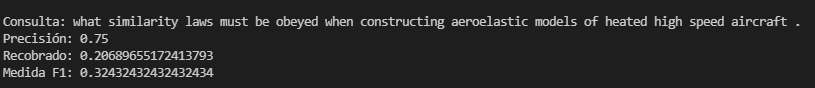
\includegraphics[height=1.3cm]{imgs/eval_query1_cran.png}
	\caption{Medidas para la primera consulta del Cranfield}
	\label{fig:cran1}
\end{figure}

Se observa la relación existente entre precisión y recobrado, para una mejor representación se emplea el grafico P/R:

\begin{figure}
	\centering
	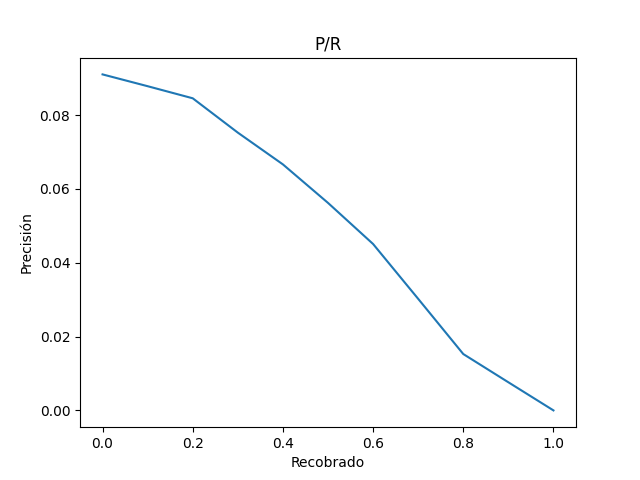
\includegraphics[height=6.3cm]{imgs/pr_query1_cran.png}
	\caption{Gráfica P/R para la primera consulta del Cranfield}
	\label{fig:cran1img}
\end{figure}

Ahora determinemos de forma general las medidas para todo el dataset de Cranfield, de esta forma sabremos el promedio de efectividad del sistema (Fig. \ref{fig:cran1gen}).

\begin{figure}
	\centering
	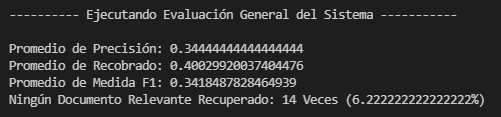
\includegraphics[height=2.3cm]{imgs/eval_general_cran.png}
	\caption{Medidas Generales para el Dataset de Cranfield}
	\label{fig:cran1gen}
\end{figure}

Estos resultados son aceptables tomando en cuenta que empleamos un modelo vectorial usando TF-IDF con algunas modificaciones, como característica extra se implementó un \textbf{query expansion} empleando WordNet que es un tesauro suministrado por NLTK, para cada término de la consulta añadíamos sus sinónimos, al realizar las pruebas al sistema se redujo los valores de precisión y recobrado debido a que para muchas consultas se determinaba un conjunto de documentos relevantes mayor al esperado, esto ocurría porque el \textbf{query expansion} incluía documentos relacionados los cuales no eran considerados relevantes para el dataset, por esta razón decidimos emplear esta mejora para mostrar sugerencias extras cuando se deseara realizar formular una nueva consulta por parte del usuario.

Ahora mostraremos los resultados para el dataset MED, el cual contiene textos sobres temas médicos, primeramente analizaremos los resultados para la consulta de prueba 27 y luego de forma general (los datos del dataset pueden ser encontrados en el código en \verb*|/dataset/MED|). La consulta 27 es la siguientes:

\begin{verbatim}
	interested in the parasitic diseases.  filaria parasites found 
	in primates, the insect vectors of filaria, the related diptera, 
	i. e.,culicoides, mosquitos, etc. that may serve as vectors of 
	this\ninfection-disease; also the life cycles and transmission of 
	the filaria.parasites and ecology of the taiwan monkey,macaca with
	cyclopis emphasis on the filarial parasite, macacanema formosana.
\end{verbatim}

Esta consulta fue seleccionada por ser bastante extensa y presentar abreviaturas, signos de puntuación dispuestos de forma no coherente, de esta forma podemos ver si el modelo TF-IDF y los métodos de preprocesado  obtienen buenos resultados. Los valores de medidas para esta son (Fig. \ref{fig:med1}) :

\begin{figure}
	\centering
	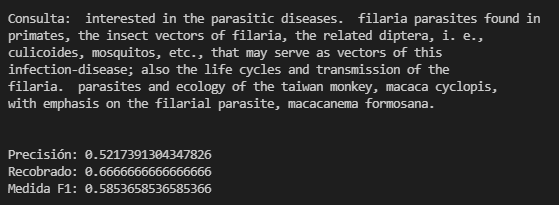
\includegraphics[height=2.5cm]{imgs/eval_query27_med.png}
	\caption{Medidas para la consulta 27 de MED}
	\label{fig:med1}
\end{figure}

Y su gráfico P/R es el siguiente (Fig. 5):

\begin{figure}
	\centering
	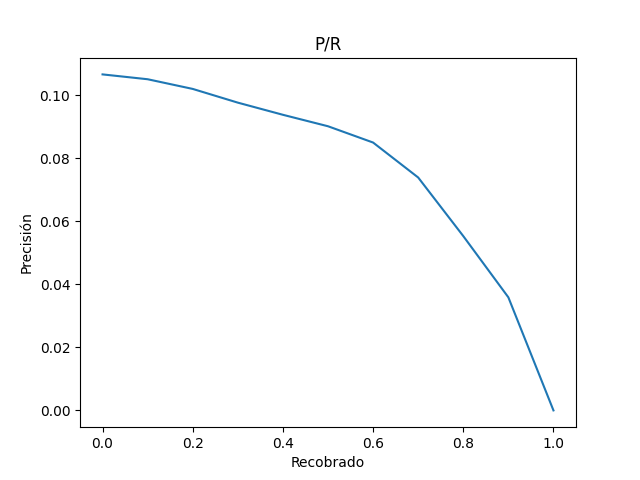
\includegraphics[height=6.3cm]{imgs/pr_query27_med.png}
	\caption{Gráfico P/R para la consulta 27 de MED}
	\label{fig:med1pr}
\end{figure}

Finalmente los valores de forma general para el dataset (Fig .6). 

\begin{figure}
	\centering
	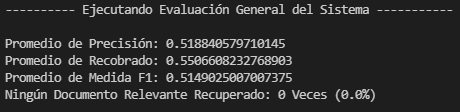
\includegraphics[height=2.3cm]{imgs/eval_general_med.png}
	\caption{Medidas Generales para el Dataset MED}
	\label{fig:med1gen}
\end{figure}

Estos resultados aunque sean mejores que los obtenidos en Cranfield, se debe tomar en cuenta la dimensión del dataset, en este caso el número de consultas y de documentos no es tan grande como el de Cranfield, además los textos son más extensos, por lo tanto a la hora de la representación es posible que se tomen características más particulares de los documentos que conforman el corpus. 

% Falta como Rocchio mejora los valores

\section{Recomendaciones}

Al analizar los resultados obtenidos y las herramientas empleadas podemos plantear algunas modificaciones y proponer el uso de otros modelos para ver el comportamiento de los resultados.

La representación vectorial usando como término una palabra no toma en cuenta ni la posición, ni las relaciones entre estos, podría realizarse un enfoque empleando modelos de Semántica Latente para agregar cierto grado de interpretación a las consultas realizadas. Adicionalmente también podríamos agregar elementos de 
similitud semántica para una mejor expansión de las consultas realizadas por el usuario.

Agregar un modelo basado en entrenamiento, tales como Regresión Logística, Árboles de Decisión o Redes Neuronales puede ayudar construir una representación más expresiva del corpus y de esta forma podríamos obtener mejores resultados. 

Por último podría emplearse términos más expresivos, el sistema emplea palabras para construir los modelos, si en lugar de palabras empleáramos n-grams o subsecuencias máximas contaríamos con entidades más completas aunque esto conllevaría a que tenga que ser modificada la representación interna, debido a que puede aumentar considerablemente la dimensión de los vectores.

\begin{thebibliography}{4}

\bibitem{confs} C. Fleitas. Sistemas de Información, Departamento de Programación, Facultad de Matemática y Computación, Universidad de la Habana, 2021

\bibitem{rocchio} J.J. Rocchio. Document Retrieval Systems–Optimization and Evaluation.
PhD thesis, Harvard Computational Laboratory, Cambridge, MA, 1966.

\bibitem{lectures} H. Yannakoudakis. Lecture 7: Relevance Feedback and Query
Expansion Information Retrieval Computer Science Tripos Part II, Natural Language and Information Processing (NLIP) Group. University of Cambridge, 2018 

\bibitem{tds} \url{https://towardsdatascience.com/} : TF-IDF in Python

\bibitem{nltk} \url{http://www.nltk.org/} : NLTK API

\end{thebibliography}

\end{document}
